% Template for PLoS
% Version 1.0 January 2009
%
% To compile to pdf, run:
% latex plos.template
% bibtex plos.template
% latex plos.template
% latex plos.template
% dvipdf plos.template

\documentclass[10pt]{article}

% amsmath package, useful for mathematical formulas
\usepackage{amsmath}
% amssymb package, useful for mathematical symbols
\usepackage{amssymb}

% graphicx package, useful for including eps and pdf graphics
% include graphics with the command \includegraphics
\usepackage{graphicx}

% cite package, to clean up citations in the main text. Do not remove.
\usepackage{cite}

\usepackage{color}

% TODO temporary
\usepackage{todonotes}

% Use doublespacing - comment out for single spacing
%\usepackage{setspace}
%\doublespacing


% Text layout
\topmargin 0.0cm
\oddsidemargin 0.5cm
\evensidemargin 0.5cm
\textwidth 16cm
\textheight 21cm

% Bold the 'Figure #' in the caption and separate it with a period
% Captions will be left justified
\usepackage[labelfont=bf,labelsep=period,justification=raggedright]{caption}

% Use the PLoS provided bibtex style
\bibliographystyle{plos2009}

% Remove brackets from numbering in List of References
\makeatletter
\renewcommand{\@biblabel}[1]{\quad#1.}
\makeatother


% Leave date blank
\date{}

\pagestyle{myheadings}
%% ** EDIT HERE **


%% ** EDIT HERE **
%% PLEASE INCLUDE ALL MACROS BELOW

%% END MACROS SECTION

\begin{document}

% Title must be 150 characters or less
\begin{flushleft}
{\Large
\textbf{Object oriented implementation of Yeadon's human inertial model}
}
% Insert Author names, affiliations and corresponding author email.
\\
Christopher Dembia$^{1,\ast}$,
Jason K. Moore$^{2}$,
Mont Hubbard$^{2}$
\\
\bf{1} Mechanical Engineering, Stanford University, Palo Alto, California, USA
\\
\bf{2} Mechanical and Aerospace Engineering, University of California, Davis, California, USA
\\
$\ast$ E-mail: Corresponding cld72@cornell.edu
\end{flushleft}

% Please keep the abstract between 250 and 300 words
\section*{Abstract}
Herein we present a modern open source software implementation of a popular
mathematical method developed by M.R. Yeadon for estimating the body segment
inertia of a human body.
% Please keep the Author Summary between 150 and 200 words
% Use first person. PLoS ONE authors please skip this step.
% Author Summary not valid for PLoS ONE submissions.
%\section*{Author Summary}

\section*{Introduction}
For dynamic analyses, it is typical to treat the human body as a collection of
linked rigid bodies. For accurate simulation and analysis the inertial
properties (mass, center of mass, and moment of inertia) of the body segments
must be estimated. Human mass, center of mass, and inertial properties have
been measured and estimated in a multitude of ways. Each method has its
advantages and disadvantages. Many methods exist including cadaver measurements
(\cite{Dempster1955}, \cite{Clauser1969}, \cite{Chandler1975}), photogrammetry,
ray scanning techniques (\cite{Zatsiorsky1983}, \cite{Zatsiorsky1990}), water
displacement (\cite{Park1999}), rotating platforms (\cite{Griffiths2005}), and
geometrical estimation of the body segments (\cite{Yeadon1990c}).
Bjornstrup \cite{Bjornstrup1995} gives a detailed overview of mostly invasive
methods up to 1995.

Yeadon's mathematical method is quite attractive as it requires only a set of
simple measurements from a live human and provides reasonable estimates of the
human's body segment parameters. Furthermore, it is based off of simple
computations and can easily be programmed to provide a quick estimate of body
segment parameters. Yeadon himself developed a Fortran program called ISEG for
his doctoral work \cite{Yeadon1984a} to rapidly compute his inertia model. The
source code is available through the dissertation under the Creative Commons
Attribution-NonCommercial-NoDerivs 2.5 license but is less than adaptable for
inclusion in modern software packages for easy configuration and visualization.

We make use of Yeadon's model extensively in our dynamics research and
developed a modern object oriented program under a permissive license that
allows for easy inclusion into software packages and includes a graphical user
interface for ease of end user use.

\subsection*{Yeadon's model}

Yeadon provides a lucid explanation of his human inertia model in
\cite{Yeadon1990c}. In this section, we merely seek to summarize his work. The
model is defined in terms of \emph{segments}, \emph{levels}, and \emph{solids}.
These three elements of the model are all shown in Figure \ref{fig:meas}.

\begin{description}
    \item[Segments]
        The human is composed of 11 segments. Each of the 4 limbs is
        composed of 2 segments, and the remainder of the body is composed of 3
        segments. Each of these segments are rigid bodies, but have at least
        one rotational degree of freedom with respect to the segment to which
        they are attached.  The segments are labeled as \textbf{C},
        \textbf{A1}, and so forth.
    \item[Levels]
        Each segment is defined by a series of parallel cross sections.
        These cross sections are referred to as levels, both in
        Yeadon's work and in ours. The model contains a toal of 45 levels.
        Levels are labeled as \textbf{Ls0}, \textbf{La0}, and so forth.  Each
        level is in the shape of a \emph{stadium} (see Figure
        \ref{fig:stadium}). The only exception to this is \textbf{Ls7} in the
        head, which is a circle. We can define a stadium by any 2 of the
        following 5 attributes: its perimeter $p$, radius $r$, thickness $t$,
        width $w$, and depth $d$.  The choice of which 2 attributes are used to
        define a given stadium depends on the stadium's location in the body,
        as, for example, it is difficult to measure a perimeter about the
        shoulders (\textbf{Ls4}) so a depth is used instead.
    \item[Solids]
        The inertial properties of each segment are computed by viewing each
        segment as a solid lofted through all the levels in the segment. This
        defines $N-1$ solids in a segment defined by $N$ levels. The solids are
        labeled as \textbf{s0}, \textbf{a0}, and so forth. All solids in a
        segment share the same longitudinal axis. A given solid is
        defined by its two bounding stadia and the longitudinal distance
        between them (the solid's height). These stadium-bounded solids are
        termed \emph{stadium solids}. The only exception is \textbf{s7}, the
        solid above the ear, which is a semi-ellipsoid. The model contains a
        total of 40 solids.  Note that in this formulation we start numbering
        the segments from 0, while Yeadon starts numbering the solids from 1.
\end{description}

A key feature of this inertia model is that it can be personalized to a given
individual, though we have not yet discussed this feature. The model is
personalized via 95 anthropometric measurements. These measurements serve to
define each stadium, and to provide the distance between the stadia (the
heights of the stadium solids).

Much of the utility of the model comes from being able to specify the
configuration of the human in which one desires its inertial properties. The configuration is specified via 21 joint angles between the various segments, all of which are
labeled in Figure \ref{fig:config}. The joint center of each segment is located
with a black dot: it is always located at the center of the base stadium of the
segment. The black arrows on each
segment indicate its local coordinate frame, whose origin is always at the
joint center of the segment. For each segment, the local $z$-axis is the longitudinal axis of the segment. The green arrows
each represent a degree of freedom, and indicate the direction and sign of the
corresponding joint angle via the right-hand rule. The configuration variables
are named with the names of the two segments at the joint, and a physiological
description of the joint angle (i.e. \verb+K1K2flexion+ is the right knee
flexion). The exceptions to this naming convention are \verb+somersalt+,
\verb+tilt+, and \verb+twist+, which specify the orientation of the whole body
with respect to the fixed coordinate frame. Thus, right hip abduction is
positive value of \verb+PK1abduction+, and so forth.

Most joints have more than one degree of freedom, but only 4 have the maximum
number of 3 rotational degrees of freedom. Since rotations are not commutative,
we must specify the order in which we perform rotations at multi-degree of
freedom joints. We provide this information in Table \ref{tab:dof}.

The default configuration is for all configuration variables to have a value of
zero. This, however, does not mean that the local coordinate basis vectors of
all segments align with the global coordinate basis vectors. In the default
configuration, the limbs (segments \textbf{A1}, \textbf{A2}, \textbf{B1},
\textbf{B2}, \textbf{J1}, \textbf{J2}, \textbf{K1}, \textbf{K2}) are rotated
$-\pi$ radians about the global $y$-axis
so that the fingers and toes point downward.

This means that for each segment, in the default configuration, the local
$x$-axis lies in a coronal plane and the local $y$-axis is directed
posteriorly. Furthermore, it is assumed that in this configuration, the palms
of the hands face the anterior direction.

\subsection*{Inertial parameters}

We provide inertial properties (mass, center of mass, and moments of inertia)
for the whole human, for an individual segment, for an individual solid, or for
any combination of segments and solids. In the first case of the whole human,
 we provide the center of mass and moments of inertia in the global fixed coordinate frame. This frame has its
 origin at the bottom middle of solid \textbf{s0}, and is aligned with the
 local frame of segment \textbf{P} when \verb+somersalt+, \verb+tilt+, and
 \verb+twist+ are zero.
 In the case of individual segments or solids, we can provide the inertial
 properties in either the local frame of the segment in inquiry, or in the
 global fixed frame. We provide the inertial properties for any other
 combination in terms of the global fixed frame.


%Yeadon's human inertia model allows one to estimate the inertial properties of a particular individual through a standard and quick process.


\todo{edit measurements figure so that we don't have <s> is hte name of the
segment, since htis is not true for the torso!! or really for any part of the
model.}



\textbf{Measurements}

It is possible that certain stadia degenerate into circles for the measurements
of a given human subject.


\subsection*{Exceptions}

-talk about exceptions in measurements
-talk about exceptions in how stadia are defined
-talk about if t is very small
-separate out exceptions in the model vs exceptions in the implementation.
-talk about negative thickness or radius.



Yeadon's mathematical model of the human body is developed by representing the
human body by a number of stadium solids and a semi ellipsoid. The ratio of the
body segment parameters are based on previous cadaver studies. He provides the
analtyical solutions for the center of mass and inertia of an individual
stadium solid. The parrlalel axis thereom is then employed to compute the
inertia properties of combinations of segments with the largest subset being
the entire body.


\todo{Talk about the number of measurements and the number of joint angles}

\section*{Software design}

The input to \verb+yeadon+ consists of (1) measurements of a subject, and (2)
the joint configuration of the subject. With these two inputs, one is able to
obtain the mass properties of the subject.
The mass properties consist of the mass, center of mass, and moment of inertia
tensor. These properties can be obtained for the entire subject, or for
individual limbs of the subject. TODO any allowable configuration.

% authors may use "Analysis"
\section*{Materials and Methods}

\section*{Usage}

We demonstrate how one may use the \verb+yeadon+ package using the example of
an ice skater performing a spin. As is commonly taught in high school physics
classes when discussing the conservation of angular momentum, an ice skater
extends her arms to spin slowly, and draws them proximally to increase her
angular velocity. Since the product $I_{zz}\omega$ remains constant and $I_{zz}$
decreases, then $\omega$ must increase (with the $z$ axis directed vertically).
We can use this human inertia model to vary a model's configuration to quickly
observe the effect on $I_{zz}$. Specifically, we want to know the factor by
which an ice skater's angular velocity may increase when she draws her arms in
from a directly outward position.

We begin by describing how \verb+yeadon+ is obtained and installed, then
discuss the two ways that \verb+yeadon+ can be used to approach this problem.

\subsection*{Obtaining and installing the software}

The package, along with its documentation, is distributed through the Python
Package Index. Accordingly, the package can be downloaded and installed easily
from the command line on a user's machine using the \verb+pip+ package:

\begin{verbatim}
$ pip install yeadon
\end{verbatim}

There are two ways to use the package: through methods of the \verb+Human+
class, or through an interactive command-line user interface. We cover both.



\subsection*{The Human class}

\begin{verbatim}
import yeadon as y
h = y.Human('female1.txt')
\end{verbatim}

This constructs the \verb+Human+ with the segment dimensions as given in the
\verb+female1.txt+ input file. This human has the default configuration, in
which all joint angles are zero. This human can be visualized by executing the
following:

\begin{verbatim}
h.draw()
\end{verbatim}
\todo{is draw() correct}

Figure \ref{fig:femaledefault} shows this Human

TODO show the use of some other methods, for instance averaging and scaling.

\subsection*{The command-line user interface}


-dev for python2.7
-assume unix machine
-dist through pip
-how to install
-two ways to use.


\todo{Measurement figure}

% Do NOT remove this, even if you are not including acknowledgments
\section*{Acknowledgments}
TODO nsf disclaimer
%\section*{References}
% The bibtex filename
\bibliography{humaninertia}

\section*{Figure Legends}
%\begin{figure}[!ht]
%\begin{center}
%%\includegraphics[width=4in]{figure_name.2.eps}
%\end{center}
%\caption{
%{\bf Bold the first sentence.}  Rest of figure 2  caption.  Caption 
%should be left justified, as specified by the options to the caption 
%package.
%}
%\label{Figure_label}
%\end{figure}

\begin{figure}[!ht]
\begin{center}
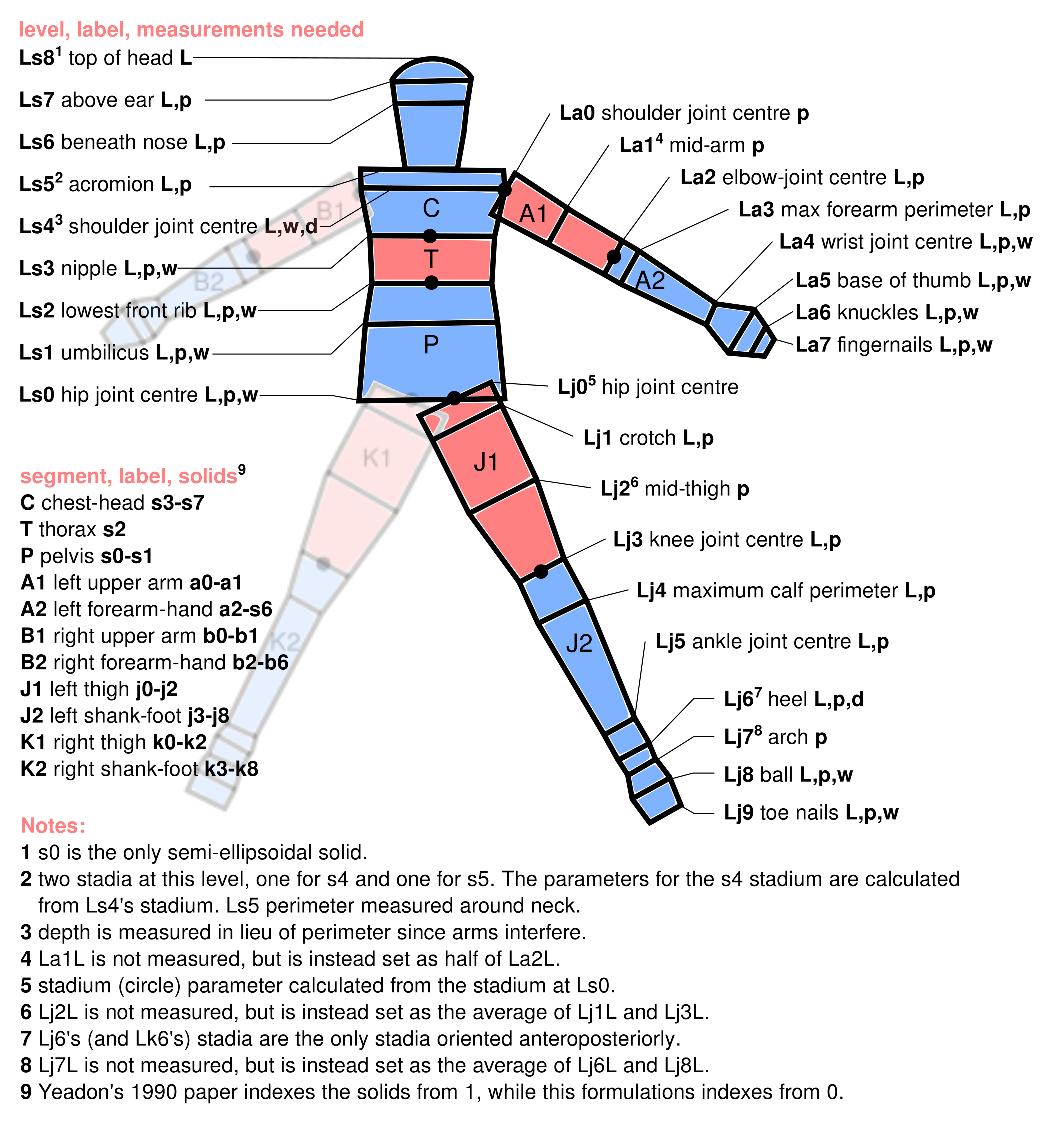
\includegraphics[width=4in]{measurements.eps}
\end{center}
\caption{
{\bf Measurements required for the human inertia model.}  The human is defined
using 95 measurements. These consist of measurements along the limbs/segments
(lengths), transverse to the limbs/segments (widths/depths), or about the
limbs/segments (perimeters) \cite{Yeadon1990c}.
}
\label{fig:meas}
\end{figure}

\begin{figure}[!ht]
\begin{center}
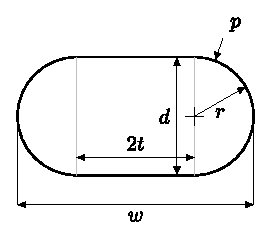
\includegraphics{stadium.eps}
\end{center}
\caption{
{\bf Stadium cross section shape.}  The levels that define the segments are all
in the shape of a stadium, with one exception. We can define a stadium by
by any two of its attributes: perimeter $p$, radius $r$, thickness $t$,  width
$w$, and depth $d$.
}
\label{fig:stadium}
\end{figure}

\begin{figure}[!ht]
\begin{center}
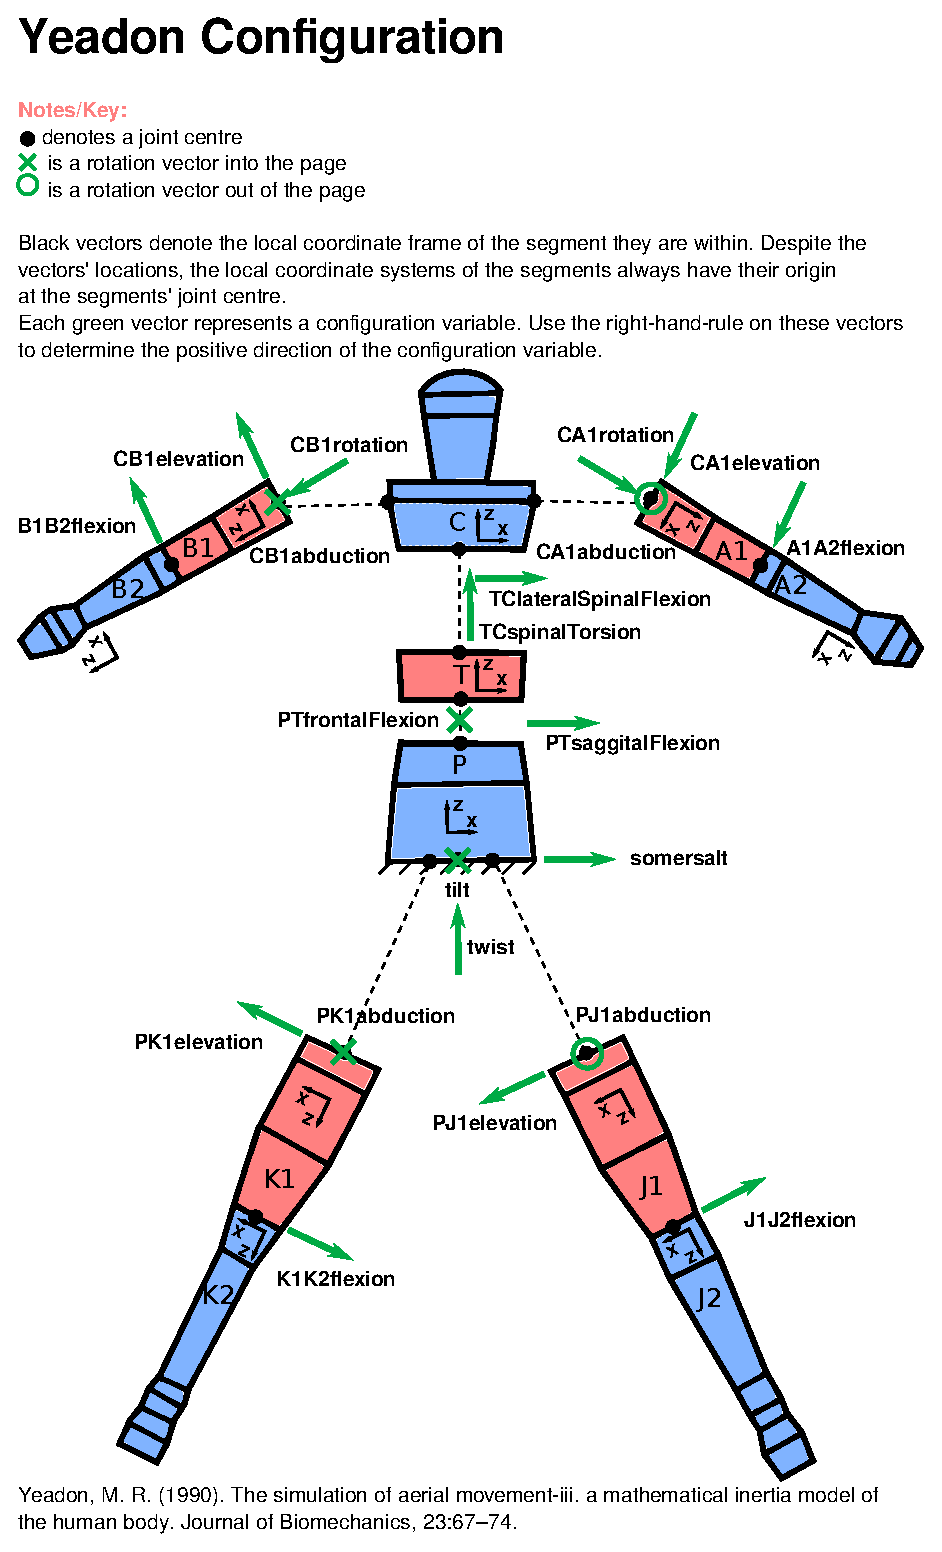
\includegraphics[width=4in]{configuration.eps}
\end{center}
\caption{
{\bf Configuration variables for the human inertia model.}  The configuration of
the human is defined using 21 joint angles, represented by green arrows
\cite{Yeadon1990e}. The labels are the names of the configuration variables in
the code. The origin of the global coordinate frame is at the bottom center of
the pelvis segment.
}
\label{fig:config}
\end{figure}

\begin{figure}[!ht]
\begin{center}
    \missingfigure{femaledefault}
%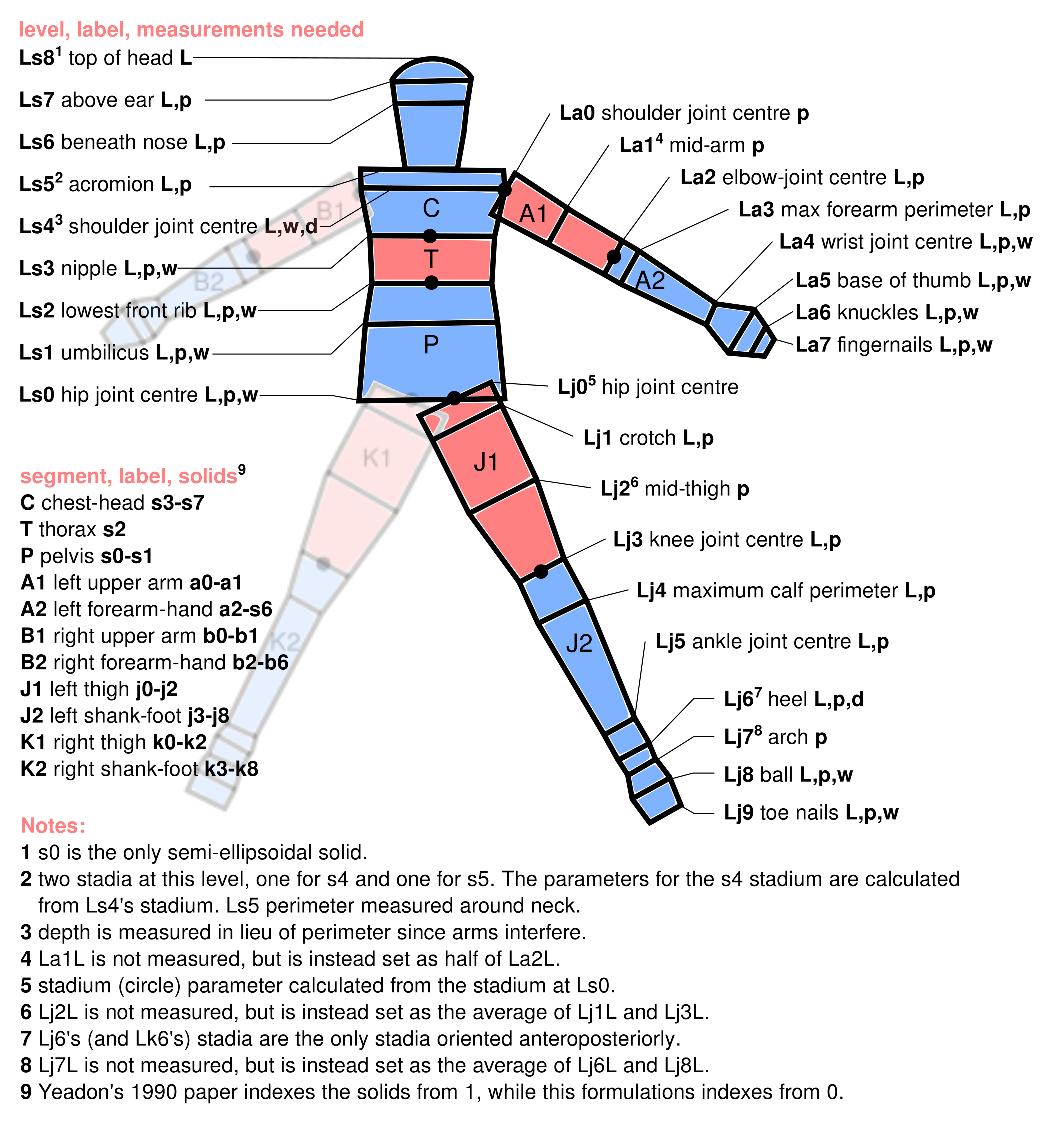
\includegraphics[width=4in]{measurements.eps}
\end{center}
\caption{
{\bf TODO Bold the first sentence.}  Rest of figure 2  caption.  Caption 
should be left justified, as specified by the options to the caption 
package.
}
\label{fig:femaledefault}
\end{figure}

\section*{Tables}
%\begin{table}[!ht]
%\caption{
%\bf{Table title}}
%\begin{tabular}{|c|c|c|}
%table information
%\end{tabular}
%\begin{flushleft}Table caption
%\end{flushleft}
%\label{tab:label}
% \end{table}

\begin{table}[!ht]
\caption{
\bf{Rotation order for multi-degree of freedom joints}}
\begin{tabular}{|c|c|}
    joint & order of rotations\\
    P & somersalt, tilt, twist \\
    PT & frontal flexion, sagittal flexion \\
    TC & TODO \\
    CA1 & elevation, abduction, rotation \\
    CB1 & elevation, abduction, rotation \\
    PJ1 & TODO \\
    PK1 & TODO \\

\end{tabular}
\begin{flushleft}Since rotations are not commutative, we must specify the order
    in which we perform rotations at multi-degree of freedom joints. For each
    joint with more than one configuration variable, we provide the order in
    which we rotate the segment with respect to the orientation of the
    preceding segment.
\end{flushleft}
\label{tab:dof}
 \end{table}


\end{document}
